\documentclass{report}

\input{preamble}
\input{macros}
\input{letterfonts}

\title{\Huge{Some Class}\\Random Examples}
\author{\huge{Your Name}}
\date{}

\begin{document}

\maketitle
\newpage% or \cleardoublepage
% \pdfbookmark[<level>]{<title>}{<dest>}
\pdfbookmark[section]{\contentsname}{toc}
\tableofcontents
\pagebreak

\chapter{}
\section{Wednesday, August 14}
\dfn{Utility}{
  Utility is the economics term for \textit{benefit}. Marginalism is the economic principle that economic decisions are made and economic behavior occurs in terms of incremental units, rather than categorically. The key insight of marginalism is that people make decisions over specific units of economic goods (economists say "at the margin"), rather than in an all-or-none fashion.
}
\dfn{How society decides how economics work}{
  \begin{itemize}
    \item What will be produced?
    \item{How will it be produced?}
    \item{Who will recieve it?}
  \end{itemize}
}
\dfn{Command Economy vs. Traditional Market Economy}{
  In a command economy the government decides every answer to all of those questions. In a market economy, the people (consumers) have complete control over the first and last answers. Companies have say over the means of production. Here's the stitch: The \textbf{Market} decides the reception in reality.
\\
There is also a mixed economy, which is somewhere on the specturm between the two extrems.\\ Pure competition is required to make a Market Economy work.
}
\thm{What does a market Economy create?}{
  \begin{itemize}
    \item Efficiency
    \item Quality
    \item principle
    \item Innovation
  \end{itemize}

}
\newpage
\section{Thursday, August 15}
\thm{PPC - Product Possibility Curves}{
   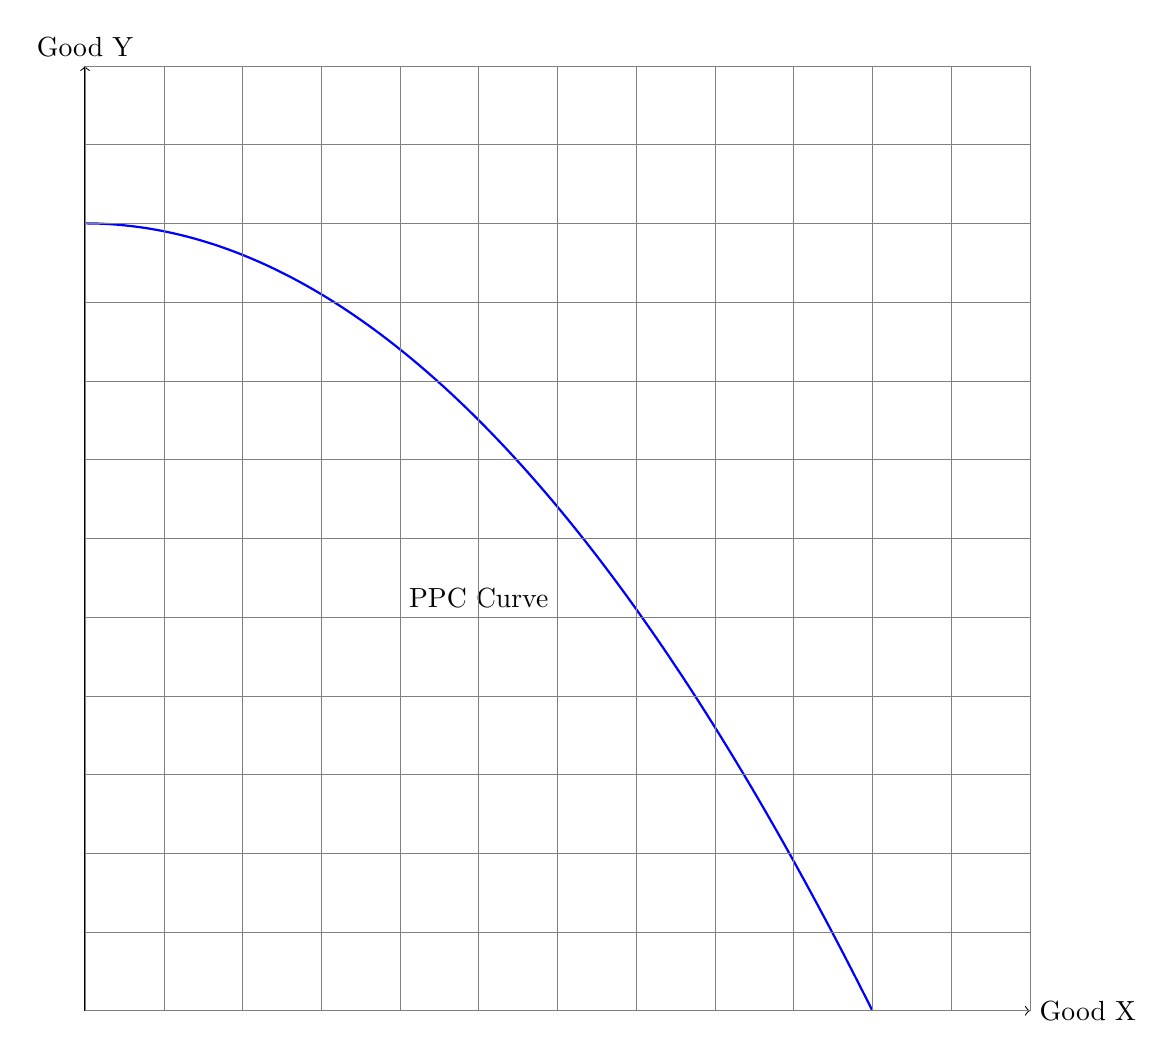
\begin{tikzpicture}
        % Draw the axes
        \draw[->] (0,0) -- (12,0) node[right] {Good X};
        \draw[->] (0,0) -- (0,12) node[above] {Good Y};
        
        % Draw the PPC curve
        \draw[thick, blue, domain=0:10] plot[variable=\x, samples=100] ({\x}, {10 - (\x^2 / 10)});
        
        % Add labels for the curve
        \node at (5, 5) [above] {PPC Curve};
        
        % Add a grid for reference
        \draw[gray, very thin] (0,0) grid (12,12);
    \end{tikzpicture}
    That is the curve of $100\%$ efficiency, if a business was working at the capacity of its infrastructure.
}

\end{document}

